\subsection{Optimization experiments} \label{supervised_approach_optim}

Here we optimize several parameters, both of the model and of the training procedure. We do so by running experiments with two values we deem reasonable for each of these parameters. The parameters we consider are dropout probability, hidden layer size and scheduler.

\subsubsection{Dropout probability}

\begin{figure}
  \begin{subfigure}[t]{.5\textwidth}
    \centering
    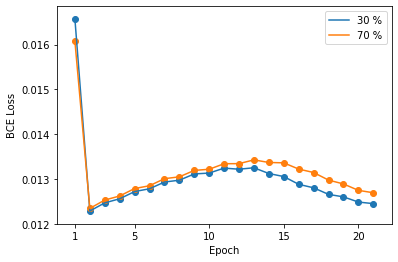
\includegraphics[width=\textwidth]{figures/supervised_approach/dropout_train_loss.png}
    \caption{Training loss}
    \label{fig:dropout_train_loss}
  \end{subfigure}
   \begin{subfigure}[t]{.5\textwidth}
    \centering
    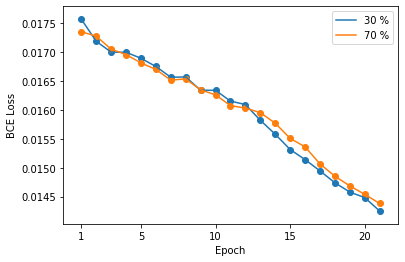
\includegraphics[width=\textwidth]{figures/supervised_approach/dropout_test_loss.png}
    \caption{Testing loss}
    \label{fig:dropout_test_loss}
  \end{subfigure}
  \caption{Test and training loss of models with different dropout probabilities.}
  \label{fig:dropout_train}
\end{figure}

\begin{figure}
  \begin{subfigure}[t]{.32\textwidth}
    \centering
    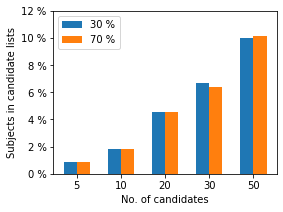
\includegraphics[width=\textwidth]{figures/supervised_approach/dropout_hw.png}
    \caption{Handwritten subjects}
    \label{fig:dropout_hw}
  \end{subfigure}
  \begin{subfigure}[t]{.32\textwidth}
    \centering
    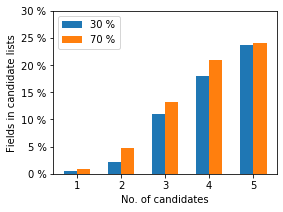
\includegraphics[width=\textwidth]{figures/supervised_approach/dropout_ddc.png}
    \caption{DDC subjects}
    \label{fig:dropout_ddc}
  \end{subfigure}
   \begin{subfigure}[t]{.32\textwidth}
    \centering
    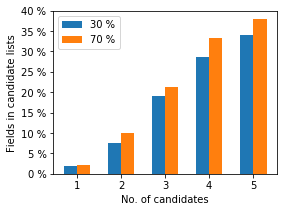
\includegraphics[width=\textwidth]{figures/supervised_approach/dropout_venue.png}
    \caption{Venues}
    \label{fig:dropout_venue}
  \end{subfigure}
  \caption{Model hit rate in the evaluation sets for different dropout probabilities.}
  \label{fig:dropout_eval}
\end{figure}

The dropout probability determines how likely it is for any element of the data to be zeroed. For instance, for a dropout probability of 50 \%, an element will be zeroed with 50 \% probability. Each element is considered independently of the rest.

In the original implementation, the authors use a dropout probability of 10 \%, which is rather low. The original proposers of dropout stated that a dropout of 50 \% is near optimal for many use cases \cite{srivastava2014dropout}. The approaches presented in chapter \ref{hmc}, which are also thematically similar to our approach, also used higher values: \cite{wehrmann2018hierarchical} uses 60 \% and \cite{giunchiglia2020coherent}, 70 \%.

For the authors of the original implementation, overfitting might not have been a threat, given that their data comprised over 11 million documents. In our case, with our smaller dataset, regularization is crucial. We therefore experiment with 50 \% and 70 \% dropout probability. Both models were trained with the same parameters, including a step-wise decaying learning rate scheduler. 

The losses during training, both throughout each epoch (figure \ref{fig:dropout_train_loss}) and on the test set (figure \ref{fig:dropout_test_loss}) are very similar during training. Although data was dropped twice as likely in one model than in the other, both models learned equally well according to the training data.

The accuracies of the models on the evaluation set are shown in figure \ref{fig:dropout_eval}. The model with less dropout seems to perform best for the handwritten subjects (figures \ref{fig:dropout_hw}), but only by a slight margin. The model with larger dropout probability performs considerably better in the other two evaluation sets, which consider the assignment of fields (figures \ref{fig:dropout_ddc} and \ref{fig:dropout_venue}, respectively).

A higher dropout probability seems to prevent overfitting, as the performance of both models is similar during training, but the one with more dropout performs better in the evaluation sets. We therefore use 70 \% as the dropout probability.

\subsubsection{Hidden layer size}

\begin{figure}
  \begin{subfigure}[t]{.5\textwidth}
    \centering
    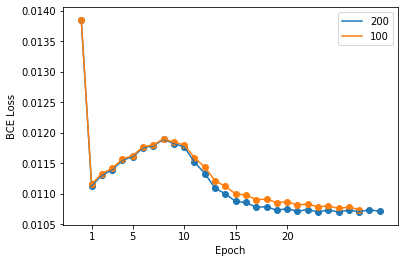
\includegraphics[width=\textwidth]{figures/supervised_approach/hidden_train_loss.png}
    \caption{Training loss}
    \label{fig:hidden_train_loss}
  \end{subfigure}
   \begin{subfigure}[t]{.5\textwidth}
    \centering
    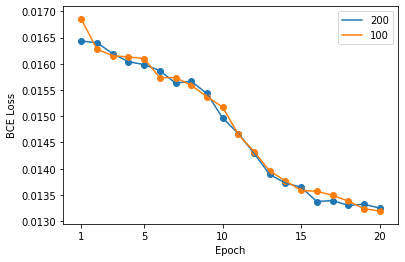
\includegraphics[width=\textwidth]{figures/supervised_approach/hidden_test_loss.png}
    \caption{Testing loss}
    \label{fig:hidden_test_loss}
  \end{subfigure}
  \caption{Test and training loss of models with different hidden layer sizes.}
  \label{fig:hidden_train}
\end{figure}

\begin{figure}
  \begin{subfigure}[t]{.32\textwidth}
    \centering
    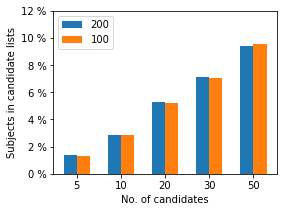
\includegraphics[width=\textwidth]{figures/supervised_approach/hidden_hw.png}
    \caption{Handwritten subjects}
    \label{fig:hidden_hw}
  \end{subfigure}
  \begin{subfigure}[t]{.32\textwidth}
    \centering
    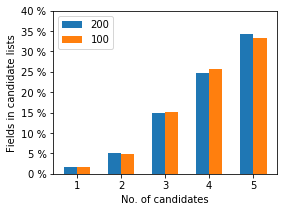
\includegraphics[width=\textwidth]{figures/supervised_approach/hidden_ddc.png}
    \caption{DDC subjects}
    \label{fig:hidden_ddc}
  \end{subfigure}
   \begin{subfigure}[t]{.32\textwidth}
    \centering
    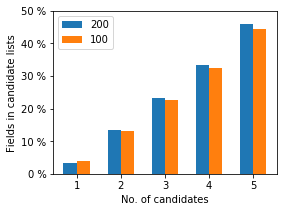
\includegraphics[width=\textwidth]{figures/supervised_approach/hidden_venue.png}
    \caption{Venues}
    \label{fig:hidden_venue}
  \end{subfigure}
  \caption{Model hit rate in the evaluation sets for different hidden layer sizes.}
  \label{fig:hidden_eval}
\end{figure}

The second parameter we experiment with is the size of the hidden layer, i.e. the size of the first fully connected layer. Its input is a one-dimensional vector of size 6,200, much smaller than the hidden layer input in the original implementation, which was over 20,000. More importantly, our set of subjects comprises 2,157 subjects, whereas the original implementation assigns 27.755 subjects to the documents. Their approach therefore requires more complexity than ours, and the hit rate of our model should not suffer with a smaller hidden layer size.

Furthermore, decreasing the complexity of the model further regularizes our pipeline, preventing overfitting. Given that the original implementation uses 1,024 nodes in the hidden layer and our set of subjects is one order of magnitude smaller than theirs, we experiment with hidden layer sizes of 100 and 200.

The training procedures are again very similar. As can be seen in figure \ref{fig:hidden_train}, both the training and testing losses of the different models are close to one another throughout all epochs. The evaluation results are also similar for both models, meaning that cutting the hidden layer size by half does not hinder the performance. Therefore, considering that the smaller size also alleviates the computational cost, we choose 100 as the hidden layer size.

\subsubsection{Learning rate schedule}

\begin{figure}
  \begin{subfigure}[t]{.5\textwidth}
    \centering
    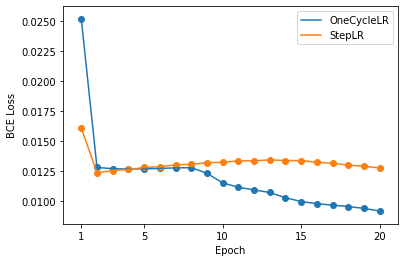
\includegraphics[width=\textwidth]{figures/supervised_approach/scheduler_train_loss.png}
    \caption{Training loss}
    \label{fig:scheduler_train_loss}
  \end{subfigure}
   \begin{subfigure}[t]{.5\textwidth}
    \centering
    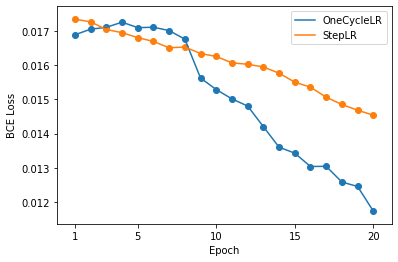
\includegraphics[width=\textwidth]{figures/supervised_approach/scheduler_test_loss.png}
    \caption{Testing loss}
    \label{fig:scheduler_test_loss}
  \end{subfigure}
  \caption{Test and training loss of models with different learning rate schedules.}
  \label{fig:scheduler_train}
\end{figure}

\begin{figure}
  \begin{subfigure}[t]{.32\textwidth}
    \centering
    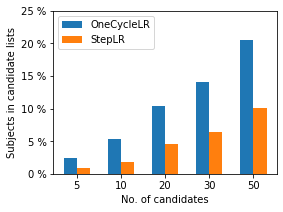
\includegraphics[width=\textwidth]{figures/supervised_approach/scheduler_hw.png}
    \caption{Handwritten subjects}
    \label{fig:scheduler_hw}
  \end{subfigure}
  \begin{subfigure}[t]{.32\textwidth}
    \centering
    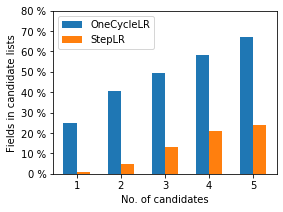
\includegraphics[width=\textwidth]{figures/supervised_approach/scheduler_ddc.png}
    \caption{DDC subjects}
    \label{fig:scheduler_ddc}
  \end{subfigure}
   \begin{subfigure}[t]{.32\textwidth}
    \centering
    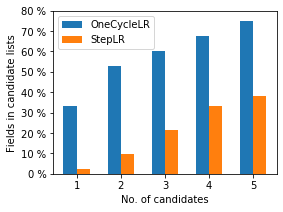
\includegraphics[width=\textwidth]{figures/supervised_approach/scheduler_venue.png}
    \caption{Venues}
    \label{fig:scheduler_venue}
  \end{subfigure}
  \caption{Model hit rate in the evaluation sets for different learning rate schedules.}
  \label{fig:scheduler_eval}
\end{figure}

\begin{figure}
    \centering
    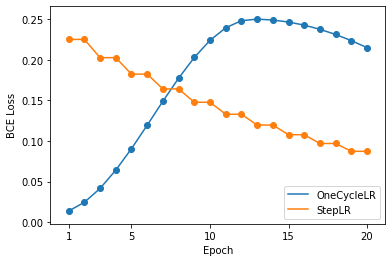
\includegraphics[width=.7\textwidth]{figures/supervised_approach/scheduler_lr.png}
    \caption{Learning rate schedules used in the experiments.}
    \label{fig:scheduler_lr}
\end{figure}

As mentioned at the beginning of this section, the original implementation uses a constant learning rate of $0.4$. Doing so is not common practice, as it is slower and does not necessarily reach optima as well as other procedures.

We have run the model with different constant learning rates to validate this assumption, and it holds: the models converge very slowly, taking small steps down the gradient, which lead to tiny loss improvements after every epoch. If we choose a higher constant learning rate, it soon starts overshooting the optimum, resulting in higher losses after a certain number of epochs.

We therefore try two learning rate schedules here. The first, called \textit{StepLR} in PyTorch, decreases the learning rate by 10 \% after every two epochs. This is the most intuitive approach: large steps are taken at the beginning, when the model is far away from its local optimal parameters. Once the model approaches the local optimum, the step size is decreased to not overshoot the optimum.

The second schedule follows the one-cycle policy, which is used in the paper where the asymmetric loss function is proposed \cite{ben2020asymmetric}. Cyclical learning rates \cite{smith2017cyclical} arise in the field of computer vision from the observation that increasing the learning rate may lead the model to perform better in the long term. The one-cycle policy, called \textit{OneCycleLR} in PyTorch, increases the learning rate until it reaches a given maximum, and then decreases it monotonically afterwards. The learning rate is updated multiple times during epochs.

Figure \ref{fig:scheduler_lr} shows both learning rate schedules across 20 epochs, both reaching a maximum learning rate of 0.25. The learning rate is updated every 100 batches in the one-cycle policy every 100 epochs, and every two epochs in the step-wise decay. The training procedures are very different from one another. The model trained with the step-wise schedule performs better in the test set (figure \ref{fig:scheduler_train_loss}) during the early epochs, where the learning rate of the one-cycle policy is still very low. However, after 10 epochs, the model trained with the one-cycle policy starts improving rapidly, being much more accurate than the other model in the end. A similar behavior can be seen in figure \ref{fig:scheduler_train_loss}, where the average training loss of each epoch is plotted.

As shown in figure \ref{fig:scheduler_eval}, the model with the one-cycle policy outperforms the one with the step-wise schedule by a very large margin, doubling its hit rate in all datasets. Especially when only one candidate is considered, it performs much better, given that the model trained with the step-wise schedule barely guesses and subjects or fields right. Thus, the three experiments we have performed show that a higher probability rate, a lower complexity and a cyclical learning rate perform best in our use case. The first two experiments indicate that regularization is important, given the differences between the documents of OpenAlex and those of the repositories.
